\section{Methods}
\subsection{Neutron reflectometry measurements}
The NR measurements analysed in this chapter were published previously by Hollinshead \emph{et al.}\autocite[full details of the experimental methods used can be found in that publication]{hollinshead_effects_2009}.
These measurements concern the study of a monolayer of 1,2-distearoyl-\emph{sn}-phosphatidylcholine\footnote{Abbreviated to DSPC.} at the air-water interface.
The NR measurements were conducted on seven isotopic contrasts of the phospholipid and water.
These contrasts were made up from four phospholipid types; fully-hydrogenated phospholipid, head-deuterated phospholipid, tail-deuterated phospholipid, and fully-deuterated phospholipid,\footnote{The different lipid constants are abbreviated to h-DSPC, \ce{d_{13}}-DSPC, \ce{d_{70}}-DSPC, and \ce{d_{83}}-DSPC respectively.} were paired with two water contrasts; fully-deuterated water and air-contrast matched water,\footnote{Abbreviated to \ce{D2O} and ACMW respectively.} where \ce{D2O} and \ce{H2O} are mixed such that the SLD is zero.
The pairing of the fully-hydrogenated phospholipid with ACMW was not performed, due to the lack of scattering available from such a system.
Measurements were conducted at four different surface pressures;\footnote{SPs.} \SIlist{20;30;40;50}{\milli\newton\per\meter}.
Table~\ref{tab:dspc} outlines the shorthands used to refer to the different contrast pairings in this work.
%
\begin{table}[t]
    \centering
    \small
    \caption{The different contrasts of phospholipid monolayer and water investigated.}
    \label{tab:dspc}
    \begin{tabular}{l | l l}
        \toprule
        Shorthand & Phospholipid contrast & Water contrast \\
        \midrule
        h-\ce{D2O} & h-DSPC & \ce{D2O} \\
        d$_{13}$-\ce{D2O} & d$_{13}$-DSPC & \ce{D2O} \\
        d$_{13}$-ACMW & d$_{13}$-DSPC & ACMW \\
        d$_{70}$-\ce{D2O} & d$_{70}$-DSPC & \ce{D2O} \\
        d$_{70}$-ACMW & d$_{70}$-DSPC & ACMW \\
        d$_{83}$-\ce{D2O} & d$_{83}$-DSPC & \ce{D2O} \\
        d$_{83}$-ACMW & d$_{83}$-DSPC & ACMW \\
        \bottomrule
    \end{tabular}
\end{table}
%

\subsection{Molecular dynamics simulations}
The DSPC monolayer simulations were made up of phospholipid molecules modelled with three potential models, each with a different degree of coarse-graining.
The Slipids potential model is an all-atom representation of the phospholipid molecules,\autocite{jambeck_derivation_2012} which was used alongside the single point charge water model,\autocite[abbreviated to SPC]{berendsen_missing_1987} with a timestep of \SI{0.5}{\femto\second}, the SHAKE, RATTLE, and PLINCS methods were used to constrain the \ce{C-H} bond.\autocite{miyamoto_settle_1992,hess_p-lincs_2008}
The Berger potential model is obtained by the integration of the hydrogen atoms into the heavy atoms to which they are bound, producing a united-atom potential model;\autocite{berger_molecular_1997} again the SPC water molecules were used.
This potential model was simulated with an increased timestep of \SI{1}{\femto\second}.\footnote{It is noted that these timesteps are shorter than those typically used for both potential models and that timesteps of up to \SI{2}{\femto\second} have been applied previously.}
Finally, the lowest resolution potential model used was the MARTINI\autocite{marrink_martini_2007} alongside the polarisable MARTINI water model,\autocite{yesylevskyy_polarizable_2010} to avoid the freezing issues observed previously.\autocite{koutsioubas_combined_2016}
The MARTINI 4-to-1 heavy atom beading allows for the use of a \SI{20}{\femto\second} timestep.
For the Slipids and Berger potential model simulations a short-range cut-off of \SI{10}{\angstrom} was used, while for the MARTINI potential model simulations the cut-off was extended to \SI{15}{\angstrom}.
All simulations were conducted with temperature coupling to a heat bath at \SI{300}{\kelvin} and a leapfrog integrator, and run using GROMACS 5.0.5\autocite{berendsen_gromacs_1995,lindahl_gromacs_2001,van_der_spoel_gromacs_2005,hess_gromacs_2008} on \num{32} cores of the STFC Scientific Computing resource SCARF.
The simulations were of monolayers, therefore the Ewald 3DC correction was applied to allow for the use of \emph{x}/\emph{y}-only periodic boundary condition.\autocite{yeh_ewald_1999}
A close-packed ``wall'' of non-interacting dummy atoms was placed at each side of the simulation cell in the \emph{z}-direction, to ensure that the atoms could not leave the simulation cell.

The starting simulation structure was generated using the molecular packing software Packmol.\autocite{martinez_packmol_2009}
This was used to produce a monolayer of \num{100} DSPC molecules, with the head group oriented to the bottom of the simulation cell.
A \SI{6}{\angstrom} layer of water was then added such that it overlapped the head groups, this was achieved with the \texttt{solvate} functionality in GROMACS 5.0.5.
Examples, of the dry and wet monolayer for the Berger potential model, can be seen in Figure~\ref{fig:drywet}.
%
\begin{figure}[t]
    \centering
    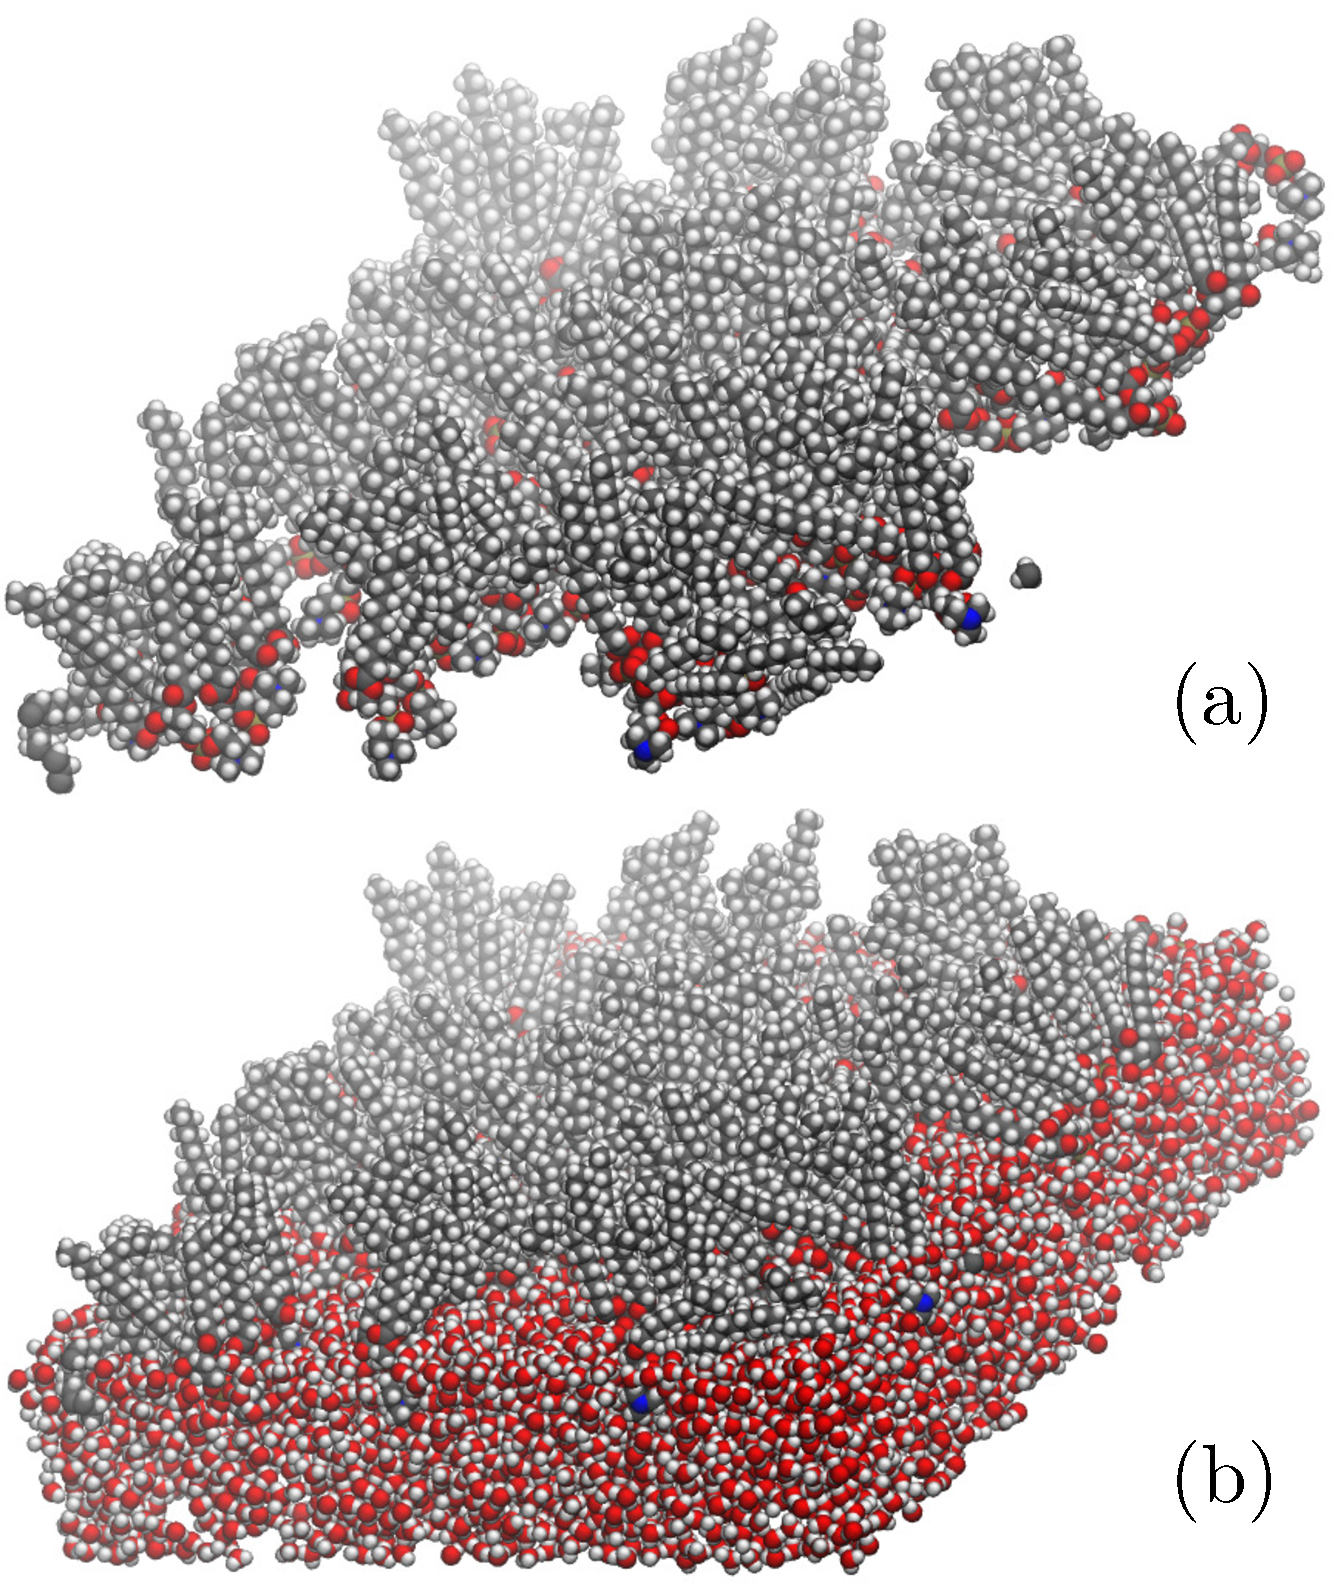
\includegraphics[width=0.60\textwidth]{reflectometry2/dspcdrywet}
    \caption{The DSPC monolayer; (a) without water layer and (b) with water layer, visuallised using VMD (\cite{humphrey_vmd_1996}).}
    \label{fig:drywet}
\end{figure}
%

A general protocol was then used to relax the system at the desired surface coverage, reproducing the effects of a Langmuir trough \emph{in-silico}.
This involved subjecting the system to a semi-isotropic barostat, with compressibility of \SI{4.5e-5}{\per\bar} of the Slipids and Berger simulations and \SI{3.0e-4}{\per\bar} for the MARTINI simulations.
The pressure in the \emph{z}-dimension was kept constant at \SI{1}{\bar}, while it was increased in the \emph{x}- and \emph{y}-dimensions isotropically.
This allowed the surface area of the interface to reduce, as the phospholipid molecules have a preference to stay at the interface, while the total volume of the system stayed relatively constant, as the water molecules move down to relax the pressure in the \emph{z}-dimension.
When the \emph{xy}-area is reached that is associated with the area per molecule\footnote{Abbreviated to APM.} for each SP, described by the experimental SP-isotherm shown in Figure~\ref{fig:surfiso} and given in Table \ref{tab:apm}, the coordinates were saved and used as the starting structure for the equilibration simulation.
This equilibration simulation involved continuing the use of the semi-isotropic barostat, with the \emph{xy}-area of the box fixed, allowing the system to relax at a pressure of \SI{1}{\bar} in the \emph{z}-dimension.
Following the application of the pair of semi-isotropic barostats, the thickness of the water layer was typically in the region of \SI{30}{\angstrom}.
The equilibration period was \SI{1}{\nano\second}, following which the \SI{50}{\nano\second} NVT\footnote{Constant number of particles, volume, and temperature.} ensemble production simulations were run, on which all analyses were conducted.
%
\begin{figure}[t]
    \centering
    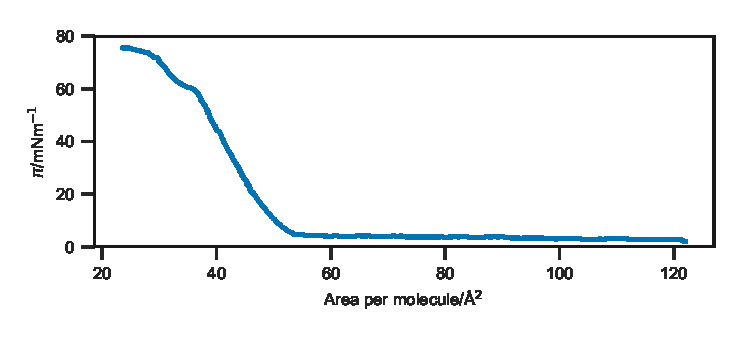
\includegraphics[width=\textwidth]{reflectometry2/apm}
    \caption{The experimental SP-isotherm for DSPC, taken from \cite{kubo_phosphatidylcholine_2001}.}
    \label{fig:surfiso}
\end{figure}
%
%
\begin{table}[b]
    \centering
    \small
    \caption{The areas per molecule (APMs) associated with particular SPs and the size of the \emph{x}- and \emph{y}-cell dimension for a simulation of 100 phospholipid molecules.}
    \label{tab:apm}
    \begin{tabular}{l | l l}
        \toprule
        $\pi$/\si{\milli\newton\per\meter} & APM/\si{\angstrom\squared} & \emph{xy}-cell length/\si{\angstrom} \\
        \midrule
        \num{20} & \num{47.9} & \num{69.1} \\
        \num{30} & \num{46.4} & \num{68.1} \\
        \num{40} & \num{45.0} & \num{67.1} \\
        \num{50} & \num{44.6} & \num{66.0} \\
        \bottomrule
    \end{tabular}
\end{table}
%
